\documentclass[12pt]{article}
\usepackage[latin9]{inputenc}
\usepackage[letterpaper]{geometry}
\geometry{verbose,tmargin=1in,bmargin=1in,lmargin=1in,rmargin=1in}
\pagestyle{plain}
\usepackage{float}
\usepackage{amsmath}
\usepackage{amssymb}
\usepackage{graphicx}
\usepackage{setspace}

% Bibliography style
\usepackage[citestyle=authoryear,natbib=true,backend=bibtex,style=chicago-authordate,
				doi=false,isbn=false,url=false]{biblatex}
%\renewcommand\nameyeardelim{, }
\bibliography{HS_pipelines.bib}

%\usepackage[authoryear,round]{natbib}


\onehalfspacing
\usepackage[unicode=true,
 bookmarks=false,
 breaklinks=false,pdfborder={0 0 1},backref=false,colorlinks=false]
 {hyperref}
\hypersetup{
 urlcolor=blue,hyperfootnotes=false,citecolor=black}
\usepackage{breakurl}

\makeatletter
%%%%%%%%%%%%%%%%%%%%%%%%%%%%%% User specified LaTeX commands.

\setcounter{MaxMatrixCols}{10}
\usepackage{graphicx}
 
\usepackage{booktabs}% Pretty tables
\usepackage{tabularx}% 
\usepackage{threeparttable}% For Notes below table
\usepackage{amsfonts}
\usepackage{multicol}
\usepackage{lscape}

\usepackage{tikz}

%\usepackage{endfloat}

\usepackage{changepage}

\usepackage{pdfpages}

\usepackage{geometry}

%\usepackage[nolists,tablesfirst]{endfloat}

\usepackage{xcolor}
\hypersetup{
    colorlinks,
    linkcolor={blue!80!black},
    citecolor={blue!80!black},
    urlcolor={blue!80!black}
}

\makeatother

%%%%%%%%%%%%%%%%%%%%%%%%%%%%%%%%%%%%%%%%%%%%%%%%%%%%%%%%%%%%%%%%%%%%%%%%%%%%%%%%%%%
% USER WRITTEN COMMENT COMMAND
% IF SELECTED, COMMAND WILL NOT DISPLAY COMMENTED TEXT  
%\newcommand{\comment}[1]{}  %comment not shown

%IF SELECTED, COMMAND WILL PRINT COMMENTED TEXT IN BLUE  
\newcommand{\comment}[1]
{{\bfseries \color{red} #1}} %comment shown

\newcommand{\inputy}[1]{\input{#1}\unskip}

%%%%%%%%%%%%%% BEGIN TEXT %%%%%%%%%%%%%%%%%%%%%%%%%%%%%%%%%%%%%%%%%%%%%%%%%%%%%%%%%%%%%%%%%%
\begin{document}

\title{Housing Market Capitalization of Pipeline Risk: Evidence from a Shock to Salience and Awareness}

\author{Evan Herrnstadt and Richard L. Sweeney\thanks{Herrnstadt: Compass Lexecon; \protect\href{mailto:eherrnstadt@gmail.com}{eherrnstadt@gmail.com}. Sweeney: Boston College; \protect\href{mailto:sweeneri@bc.edu}{sweeneri@bc.edu}. Code for replication available at \url{https://github.com/rlsweeney/public_HS_pipelines}. This work has been supported by the Sloan Foundation, Harvard Environmental Economics Program, Consortium for Energy Policy Research at Harvard, Belfer Center for Science and International Affairs, and NBER Hydrocarbon Infrastructure and Transportation workshop. We thank Jackie Glasheen and Jean-Francois Gauthier for excellent research assistance. Thanks to Kate Konschnik, Nick Kuminoff, Erzo Luttmer, and participants of various seminars for helpful comments. The views herein are the views of the authors and do not reflect or represent the views of Compass Lexecon.}}
\maketitle
\begin{abstract}
Stated safety concerns are a major impediment to making necessary expansions to the natural gas pipeline network. While revealed willingness to pay to avoid existing natural gas pipelines appears small, it is difficult to know if this reflects true ambivalence or a lack of salience and awareness. We test this latter hypothesis by studying how house prices responded to a deadly 2010 pipeline explosion in San Bruno, CA, which shocked both attention and information. Using multiple identification strategies, we fail to find any evidence of a meaningful shift in the hedonic price gradient around pipelines following these events. We conclude that the safety costs imposed by natural gas pipelines are likely small, consistent with rational expectations.

\vspace{1cm}

Keywords: Hedonic; Pipeline; Safety; Information Disclosure

JEL Codes: Q4, Q5, Q51, R21

\vspace{1cm}

\pagebreak{}
\end{abstract}

\section{Introduction}

Due to advances in drilling technology, the economically recoverable supply of natural gas in the United States nearly doubled between between 2005 and 2014.\footnote{Source: \href{https://www.eia.gov/naturalgas/crudeoilreserves/}{https://www.eia.gov/naturalgas/crudeoilreserves/}.} In order to fully capture the benefits of this unexpected resource boom, significant increases in and improvements to the existing pipeline network are required. Despite this, according to the regulatory body which oversees these changes, the Federal Energy Regulatory Commission (FERC), new pipelines ``are facing unprecedented opposition from local and national groups''.\footnote{FERC Commissioner Cheryl LaFleur (1/27/2015), \href{https://www.ferc.gov/media/videos/lafleur/2015/012715-lafleur.pdf.}{https://www.ferc.gov/media/videos/lafleur/2015/012715-lafleur.pdf.} } A major source of this opposition, particularly in densely populated areas, is concern about pipeline safety \citep{parfomak_keeping_2013,parfomak_dots_2016}. Efficient infrastructure policy would weigh these safety concerns (and other costs) against the benefits of more transmission.\footnote{There is abundant evidence which suggests these benefits could be large, at least in the short run. Due to plant closures, New England's electric power grid is increasingly reliant on natural gas. This past winter, due to transmission constraints, New England states had the four highest electricity prices in the continental United States  (and six of the top eight) (EIA State Energy Data System, accessed April 1, 2019). In Westchester County, New York, gas utility Con Ed recently implemented a moratorium on new residential natural gas hookups in response to supply constrains (``Con Ed Cuts Off New Gas Hookups in New York Suburb,'' \textit{The New York Times} March 21, 2019)}
%\href{https://www.eia.gov/state/rankings/?sid=MA#series/31}

Placing a value on the safety costs of pipelines is challenging. If we consider risk of death alone, natural gas pipelines are extremely safe: over the past two decades, incidents along the United States' 300,000 mile transmission network have resulted in an average of only 2.3 deaths per year.\footnote{Over the 20-year period of 1995\textendash 2014, local distribution system accidents accounted for 279 fatalities and more than 1,000 injuries, while transmission systems accounted for 42 fatalities and 174 injuries, or about one-seventh of the total. Over the 4-year period of 2011\textendash 2014, there has only been one single transmission-related fatality  (\citealp{united_states_department_of_energy_quadrennial_2015}, pp NG-54).} However, when they occur, pipeline explosions are horrific.\footnote{In addition to the incident studied in this paper, other prominent recent explosions include Allentown, PA in 2011, where four adults and a toddler were killed, and Massachusetts in 2018, where a Columbia Gas leak caused the emergency evacuation of several Boston suburbs.} If individuals are particularly fearful of this risk, a simple benefit transfer using VSL could substantially understate the true disamenity.\footnote{Psychology and behavioral economics provide numerous reasons why the disamenity associated with this particular risk might exceed that captured by a more typical VSL estimate \citep{kahneman_judgment_1982}. People generally overestimate the likelihood of risks that are uncontrollable, catastrophic, and inequitably distributed \citep{slovic_perception_1987}, and exhibit probability neglect regarding fearsome risks \citep{sunstein_overreaction_2011}. A long literature documents evidence where individuals \citep{gayer2000private} and regulators \citep{viscusi1999risk} appear to \textit{overvalue} such risks.} In theory, a contingent valuation study could elicit valuations which reflect the full extent of individuals' safety concerns \citep{carson_contingent_2012}. However, in the case of pipelines, where it is clear that no payment will ever actually take place, local groups that are even modestly inconvenienced have an incentive to overstate their willingness to pay. 

A revealed preference approach, comparing house prices near to and far from pipelines has the potential to address both these concerns, but entails other challenges. First, pipelines are not randomly located, so we need quasi-experimental variation to distinguish their effect from that of any other correlated unobservables that also affect home prices \citep{parmeter_quasi-experiments_2013}. A second, less common, concern arises from the fact that people are generally uninformed about or inattentive to the existing pipeline network. Existing pipelines are hidden underground and not well marked, and detailed maps were made intentionally difficult to access after the terrorist attacks of September 11, 2001. As a consequence, when \citet{hansen_environmental_2006} asked homeowners known to live near pipelines how close they thought they were, 55 percent flatly denied living near one. If people are not mindful of or even able to locate existing pipelines, it will be very difficult to infer their true aversion to this disamenity from house price data.\footnote{There is also some survey evidence consistent with this. \citet{brogan_evaluating_2017} conducted a survey of 738 individuals, and found that respondents randomly provided with additional information about pipeline risks and a salient account of a recent pipeline incident were significantly more likely to oppose pipeline expansion.} 

In this paper, we leverage this general lack of pipeline awareness to look for a shift in the relationship between house prices and pipeline proximity following one of the deadliest pipeline incidents in U.S. history. On September 9th, 2010, a 30-inch transmission pipeline owned by Pacific Gas and Electric (PG\&E) exploded in a densely populated suburb of San Francisco, killing eight people. The event generated prolonged media coverage, particularly in the state of California, bringing the issue of pipelines to the forefront of people's minds. In the weeks that followed, outrage swelled over the lack of pipeline location information. It was revealed that, incredibly, even the local fire chief was unaware of the high pressure pipeline's presence before it exploded. The following spring, in response to this outrage, PG\&E sent letters out to all households living within 2000 feet of a pipeline alerting them to their proximity.

To test whether this shock to pipeline awareness and location information affected people's revealed preferences for living near pipelines, we look for changes in the hedonic price gradient following these events. We combine data on the universe of housing transactions in California with a proprietary map containing a snapshot of all natural gas transmission pipelines in the state. Our main approach is a difference-in-difference (DD) strategy that compares housing transactions within 1000 or 1000-2000 feet from a pipeline to those between 2000 and 4000 feet away. Leveraging the size of our sample to finely control for differential trends in narrow geographic housing markets, we compare the price gradient after the explosion and informational letter to the pre-explosion equilibrium. 

Using a variety of different temporal and spatial controls, we find no evidence that either the explosion or the letter was capitalized into house prices. This result is robust to limiting our analysis to just the counties immediately surrounding San Bruno, and to triple-difference comparisons against other properties near pipelines in southern California. Using a regression discontinuity design, we also fail to find evidence of a spatial break in the hedonic price gradient at the 2000-foot cutoff for receiving the informational letter. 

Given the nature of the variation generated by San Bruno and the reduced-form estimation strategy used, we are not able to recover (or even bound) fully informed, attentive willingness to pay (WTP) to avoid living near a natural gas pipeline without making additional assumptions. Borrowing notation from the energy efficiency gap literature \citep{allcott_is_2012}, we show that the coefficient on our DD estimator is equal to the product of the change in pipeline awareness and the true, fully informed, price relationship. After providing evidence that households were uninformed before the explosion, and that the ensuing events meaningfully increased attention and awareness, we conclude that the second term in that product must be small to generate our estimates. We conclude by demonstrating that this non-response is consistent with a rational assessment of pipeline risk valued at VSL. 

This precise null result has important policy implications. There are more than 5,000 miles of natural gas transmission pipelines currently under consideration in the United States, and industry groups predict that over 20,000 additional miles will be added by 2035.\footnote{Pending pipelines based on the list of proposed pipeline projects maintained by the Energy Information Administration. Spreadsheet of projects available at \href{https://www.eia.gov/naturalgas/data.php\#pipelines}{https://www.eia.gov/naturalgas/data.php\#{}pipelines} (accessed 4/29/2018). Projected additions taken from a 2016 study prepared for the INGAA Foundation  \citep{icf_international_north_2016}. } This increase in demand has been met with increased opposition and challenges to the siting process \citep{tierney_natural_2017}. To date, the valuation methods employed by both sides have been less than ideal, either focusing too narrowly on only houses lying in the pipeline right of way or using dubious valuation approaches.\footnote{For example, FERC's recent environmental impact statement for the approved Atlantic Coast Pipeline relied primarily on "comparables" studies, which ask appraisers to value houses with and without pipelines on them (Atlantic Coast Pipeline and Supply Header Project Final Environmental Impact Statement, July 2017, \href{https://www.ferc.gov/industries/gas/enviro/eis/2017/07-21-17-FEIS/volume-I.pdf}{FERC/EIS-0274F}, page 4-504). An opposition study submitted as comment to the same pipeline docket found that 68 percent of realtors surveyed believed a pipeline would reduce nearby properties by 5 to 10 percent \citep{phillips_economic_2016}. This latter study also analyzed 1299 resident comment letters submitted to the FERC docket; of those, 521 mentioned property values and 517 expressed a belief that the pipeline would reduce property values.} In contrast, this study leverages plausibly exogenous variation to study revealed aversion to pipelines from tens of thousands of housing transactions across the entire potential blast zone.\footnote{One noteworthy recent paper with a plausible causal strategy is \citet{BOSLETT2019}, which finds a remarkably large (9 percent) decline in home prices near a proposed (never built) New York pipeline following it's announcement.} 

More broadly, this paper contributes to a growing literature on the the relationship between house prices and energy infrastructure, such as natural gas wells \citep{muehlenbachs_housing_2015} and power plants \citep{davis_effect_2010}. One closely related study, examined housing prices in the aftermath of a gasoline pipeline explosion in Bellingham, WA in 1999, which killed three people \citep{hansen_environmental_2006}. While the paper finds that houses closer to the pipeline sold at a discount after the explosion but not before, there is no formal test of the difference between these coefficients. In addition, areas near the pipeline may have been adversely affected due to the loss of nearby parkland to the ensuing fire. In our context, we consider the impact on houses in the ``shadow'' of pipelines much further away that could not have been affected by the direct disamenity of the San Bruno explosion.

This paper also contributes to the empirical literature exploring the impact of imperfect information and inattention on hedonic models. Inattention or imperfect information has been shown to lead to suboptimal purchases in many settings \citep{chetty_salience_2009}. \citet{pope_buyer_2008} was one of the first papers to explicitly discuss how asymmetries in buyer and seller information can affect the hedonic price gradient and complicate analysis. A number of other papers have expanded upon this empirically, testing how information disclosure pertaining to toxic releases \citep{mastromonaco_environmental_2015} or underground storage tanks \citep{guignet_what_2013} are capitalized into home values. At the other extreme, several papers have demonstrated that people appear to \emph{over-react} to recent disasters, then eventually forget about them. For instance, \citet{gallagher_learning_2014} shows that flood insurance takeup spikes immediately after a flood, but decays quickly. \citet{TANAKA2018411} show a large decrease in housing prices near nuclear plants in the United States in the aftermath of the Fukushima meltdown, but this effect decayed fully within one year.\footnote{In contrast, \citet{ANDO201713} find no response from a similar exercise in Sweden.}

The rest of this paper proceeds as follows. Section \ref{sec: pipelines} provides an overview of the natural gas pipeline system and the events in California related to and following the San Bruno pipeline explosion. Section \ref{sec:Data} describes the data, Section \ref{sec:Empirical-strategy} discusses our various empirical strategies, and Section \ref{sec:Results} presents the results. Sections \ref{sec:Discussion} and \ref{sec:Conclusion} discuss policy and other implications and conclude.

\section{Background\label{sec: pipelines}}

\subsection{Natural Gas Pipelines}

For all intents and purposes, pipelines are the only real option for
transporting natural gas from the wellhead to the end-user.\footnote{While an increasing amount of natural gas being shipped as liquefied
natural gas (LNG) on enormous tankers, the costs of liquefaction are
prohibitively high except on very large scales in the presence of
substantial price differentials. } This stands in contrast to crude oil, where pipelines compete with barge and railway shipping. There are three main types of natural gas pipelines: gathering, transmission, and distribution. Gathering
pipelines are found in the producing region, and collect gas from
the wellhead and ship it a processing plant. Transmission lines then
send large quantities of processed natural gas to demand centers.
Because of the distance and volume involved, these pipelines are larger
in diameter (20-42 inches) and operate at much higher pressure than
gathering or distribution lines. Once the gas has reached its destination,
the gas is depressurized. Some of the gas will be delivered directly
to industrial customers or electricity generation facilities. Residential,
commercial, and some industrial users are serviced by distribution
pipelines. These pipes are much smaller in diameter and operate at
low pressure.

This paper focuses on transmission pipelines, which carry large quantities
of gas at very high pressure. There are over 300,000 miles of natural
gas transmission lines in the United States, but recent upstream and
downstream shocks have prompted a wave of expansion requests. Due to
the advent of hydraulic fracturing and horizontal drilling, annual
U.S. natural gas production increased by 50 percent over the past
decade, with much of the increase coming from new geographic regions
rather than existing conventional basins.\footnote{This trend is expected to continue, with annual domestic natural gas
production increasing from a current level of 27 tcf to 45 tcf in
2050 in the Energy Information Administration's 2018 Annual Energy
Outlook. } On the demand side, retiring coal-fired and nuclear power plants
are increasingly being replaced by natural gas generators, further
stressing the existing pipeline network. In response to these developments, thousands
of miles of new and expanded natural gas transmission pipelines have
been proposed. The Department of Energy projects that \$42 billion
will be spent on expanding natural gas pipeline infrastructure during
2015-2030 \citep{united_states_department_of_energy_quadrennial_2015}. 

Interstate natural gas pipelines are regulated by the Federal Energy
Regulatory Commission (FERC). They are granted power of eminent domain,
but must meet the requirements for a Certificate of Public Need. The
approval process typically involves an environmental impact statement
or assessment, a public comment period, and public meetings. This
process, along with easement negotiations, will inform local residents
about the construction plans, future existence of the pipeline, and
may prompt further information acquisition. 

The information available and attention given to pipelines during
the siting process declines considerably once they are in operation.
As a recent review on the subject concluded, ``Americans often pay
little attention at all to the nation's energy infrastructure until
they face a nearby pipeline leak, rail accident, or other natural
or man-made disaster'' \citep{klass_transporting_2014}. Part of
this is because pipelines are not well marked unless necessary. Further,
obtaining information on pipeline location was made more difficult
by the advent of the Critical Energy Infrastructure Information (CEII)
designation following 9/11. Although FERC revised its rules in 2006
to exclude purely locational information from the CEII designation,
the only publicly available source of information on transmission
pipeline location remains the National Pipeline Mapping System (NPMS).
This website does not allow one to download spatial data, view more
than one county at a time, or resolve the location of pipelines beyond
a 500 foot tolerance. The only individuals allowed to access the database
directly are government employees (who may access pipeline data under
their jurisdiction) or pipeline operating companies (who may access
data about their own pipelines).

\subsection{The San Bruno Explosion and Aftermath}

On September 9, 2010, a segment of 30-inch diameter PG\&E transmission
pipeline 132 exploded in the middle of the Crestmoor neighborhood
in San Bruno, CA. Eight people were killed, 38 homes were destroyed,
and an additional 70 homes had major or minor damage as a result of
the explosion and fire.\footnote{ Appendix Figure \ref{fig:sanbruno} provides a sense of the scale
of the damage.} The explosion occurred when an electrical glitch led to an increase
in pressure, which blew open an existing welding flaw. In the aftermath
of this disaster, PG\&E was fined \$1.6 billion by the California
Public Utilities Commission, paid out over \$565 million in civil
settlements, and was eventually found guilty of six criminal counts
in federal court.\footnote{See, respectively, ``PG\&E slapped with record \$1.6 billion penalty
for fatal San Bruno explosion'' (April 9, 2015); ``San Bruno blast:
PG\&E settles nearly all remaining lawsuits for a \$565 million total''
(Sept. 9, 2013); and ``PG\&E loses ruling in San Bruno explosion
trial'' (Nov. 17, 2016); all in the \emph{San Jose Mercury News}.}

Media coverage of the disaster was widespread, and often focused on
the existence of pipelines running locally along major roads or through
neighborhoods.\footnote{For example: ``PG\&E Says the Valley has 4 High Risk Gas Pipelines'',
\emph{KMPH News} (Sept. 21, 2010); ``Natural gas transmission lines
run near Highway 101 in Marin'', \emph{Marin Independent Journal}
(Sept. 13, 2010); ``Pipeline in San Bruno blast runs through Palo
Alto'', \emph{Palo Alto Online} (Sept. 20, 2010).} Shortly after the incident, PG\&E was pressured to release a list
outlining the 100 pipeline segments of highest priority for maintenance
and monitoring. Although this list was generated using a number of
criteria, the press coverage dubbed these segments the 100 ``riskiest''
pipeline segments, generating further publicity for the location of
natural gas transmission pipelines throughout Northern California.
In November 2010, one community in Northern Sacramento even closed
an elementary school mid-year after discovering that it was near PG\&E
pipelines and natural gas storage tanks.\footnote{``Quick closure of N. Sacramento school debated'', \emph{Sacramento
Bee} (Nov. 20, 2010).}

The spike in attention suggested by these anecdotes about media coverage
are backed up by Google search activity. We collected Google Trends
data on searches for stories that Google has determined are related
to the San Bruno pipeline explosion. Figure \ref{fig:googletrends}
displays search activity for this set of stories over time, relative
to the overall level of search activity in the geographic area.\footnote{That is, these numbers can be interpreted as the ``search rate'',
and are comparable across search terms and/or geographies within a
given graph. } In the first graph, we compare search rates in various media markets.
All three major California markets saw substantial search activity,
though LA was less affected. New York City also shows some activity,
suggesting that, while this was a major national news story, it got
disproportionate attention in California. 

\begin{figure}[H]
\caption{Google search rates\label{fig:googletrends}}

\centering
\begin{centering}
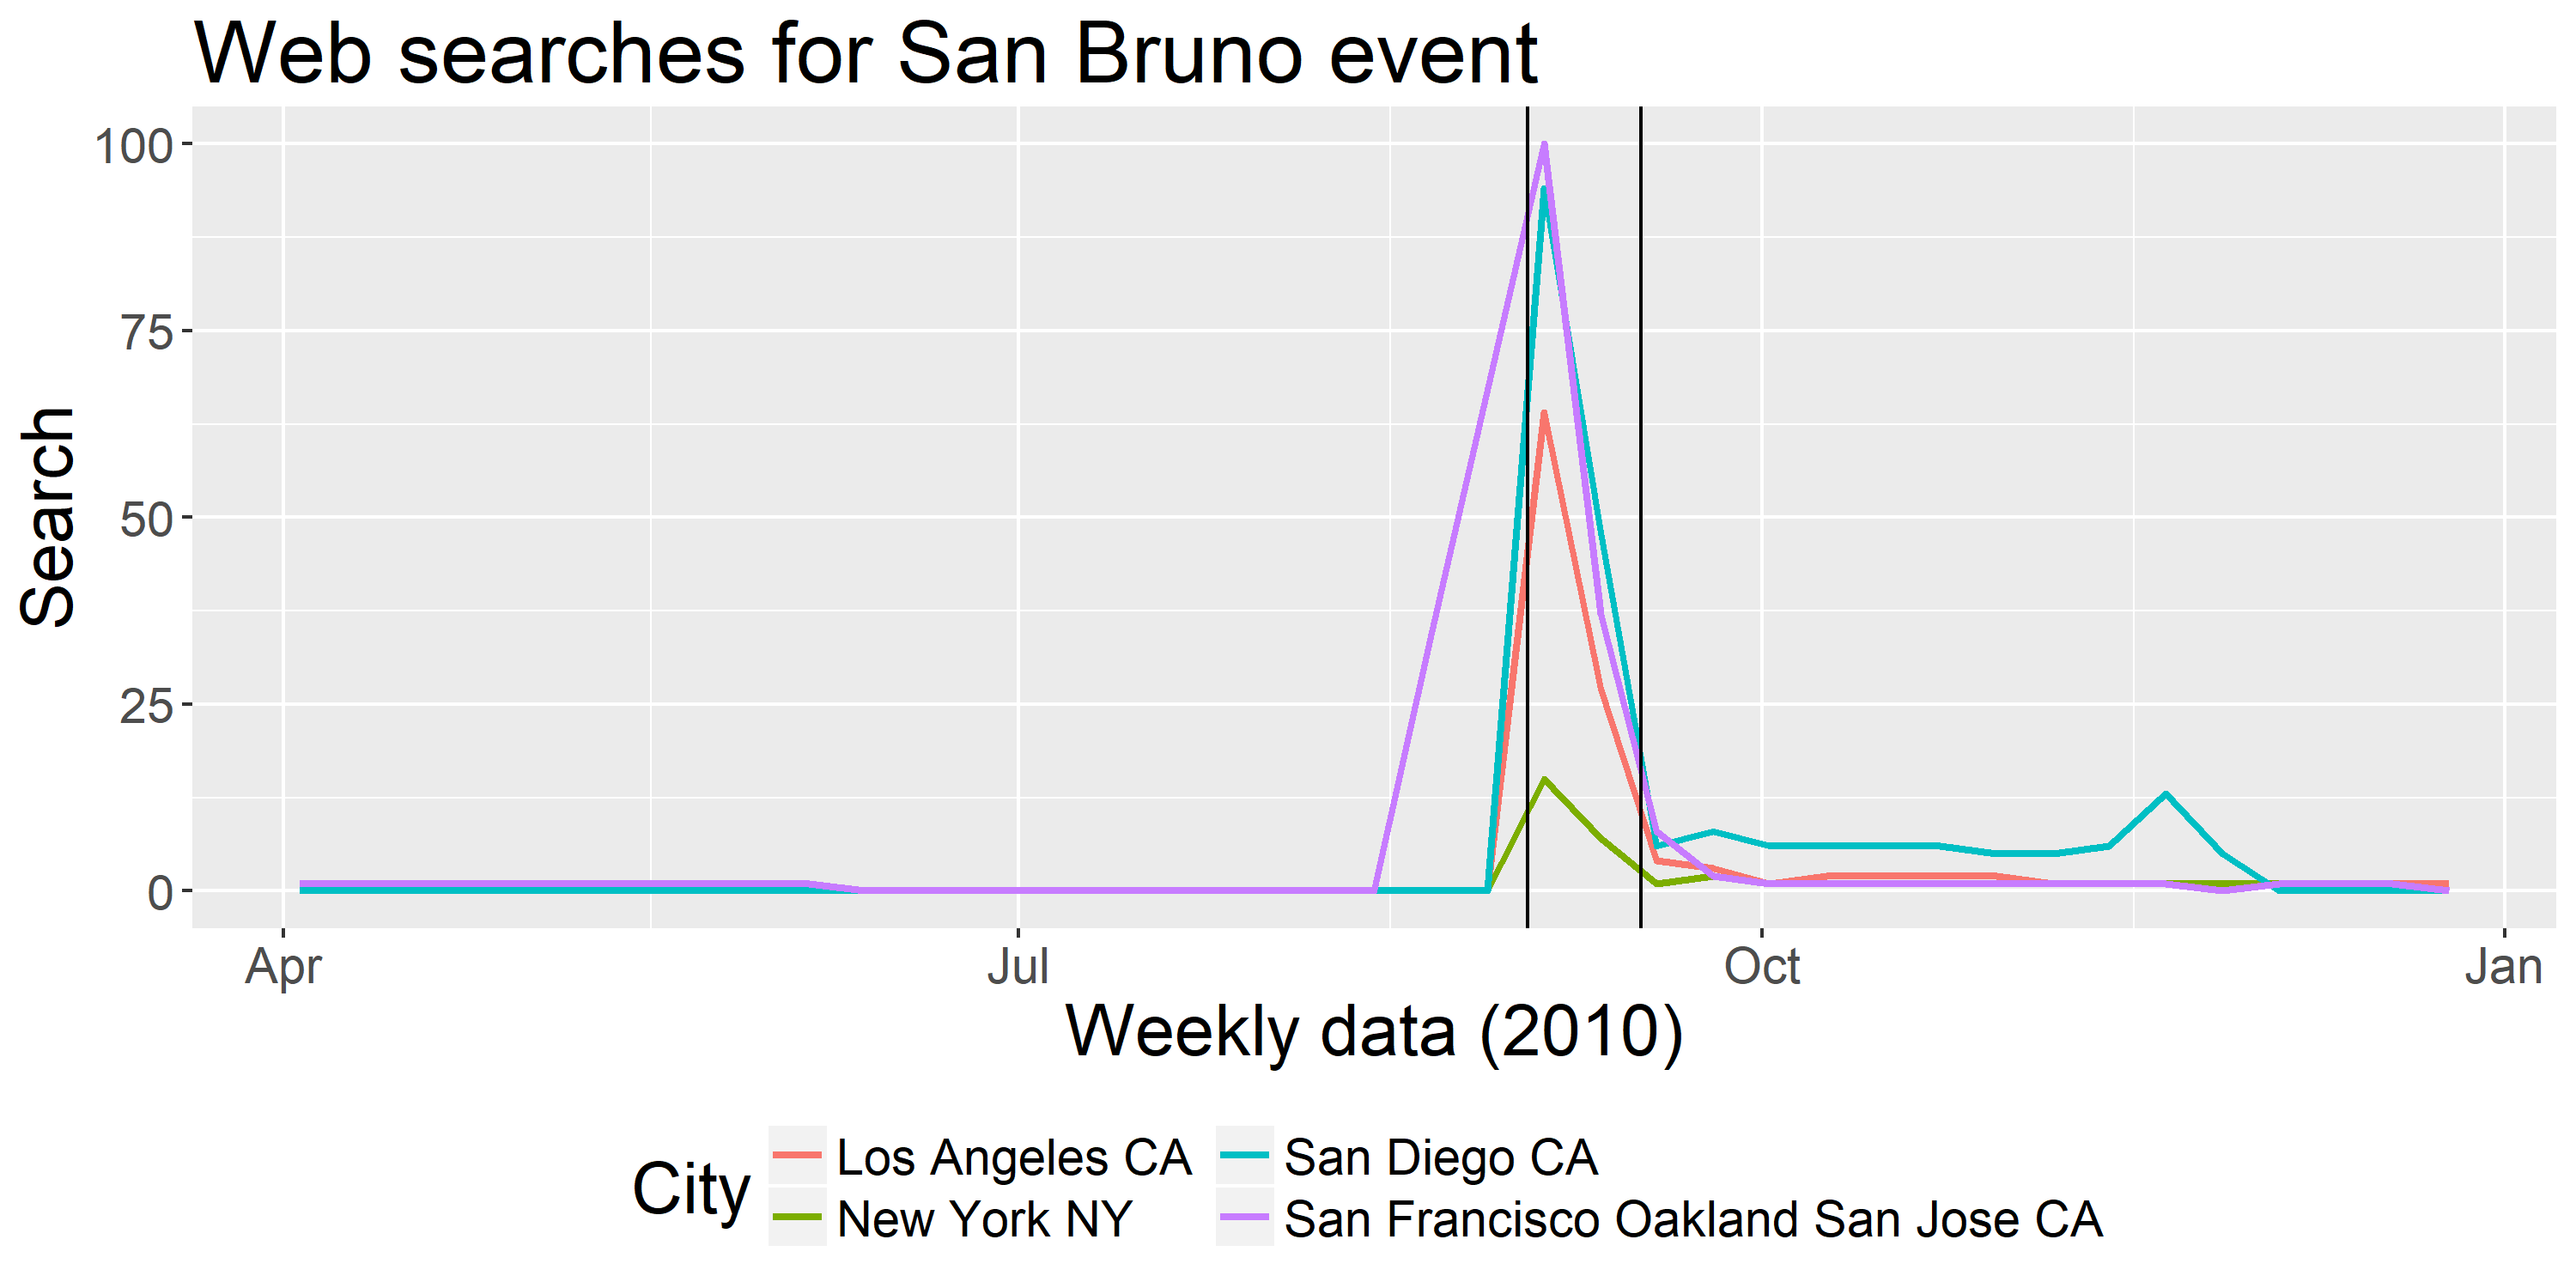
\includegraphics[width=0.75\textwidth]{../output/google_sanbruno_cities_web.png}
\par\end{centering}
\vspace{3ex}
\begin{centering}
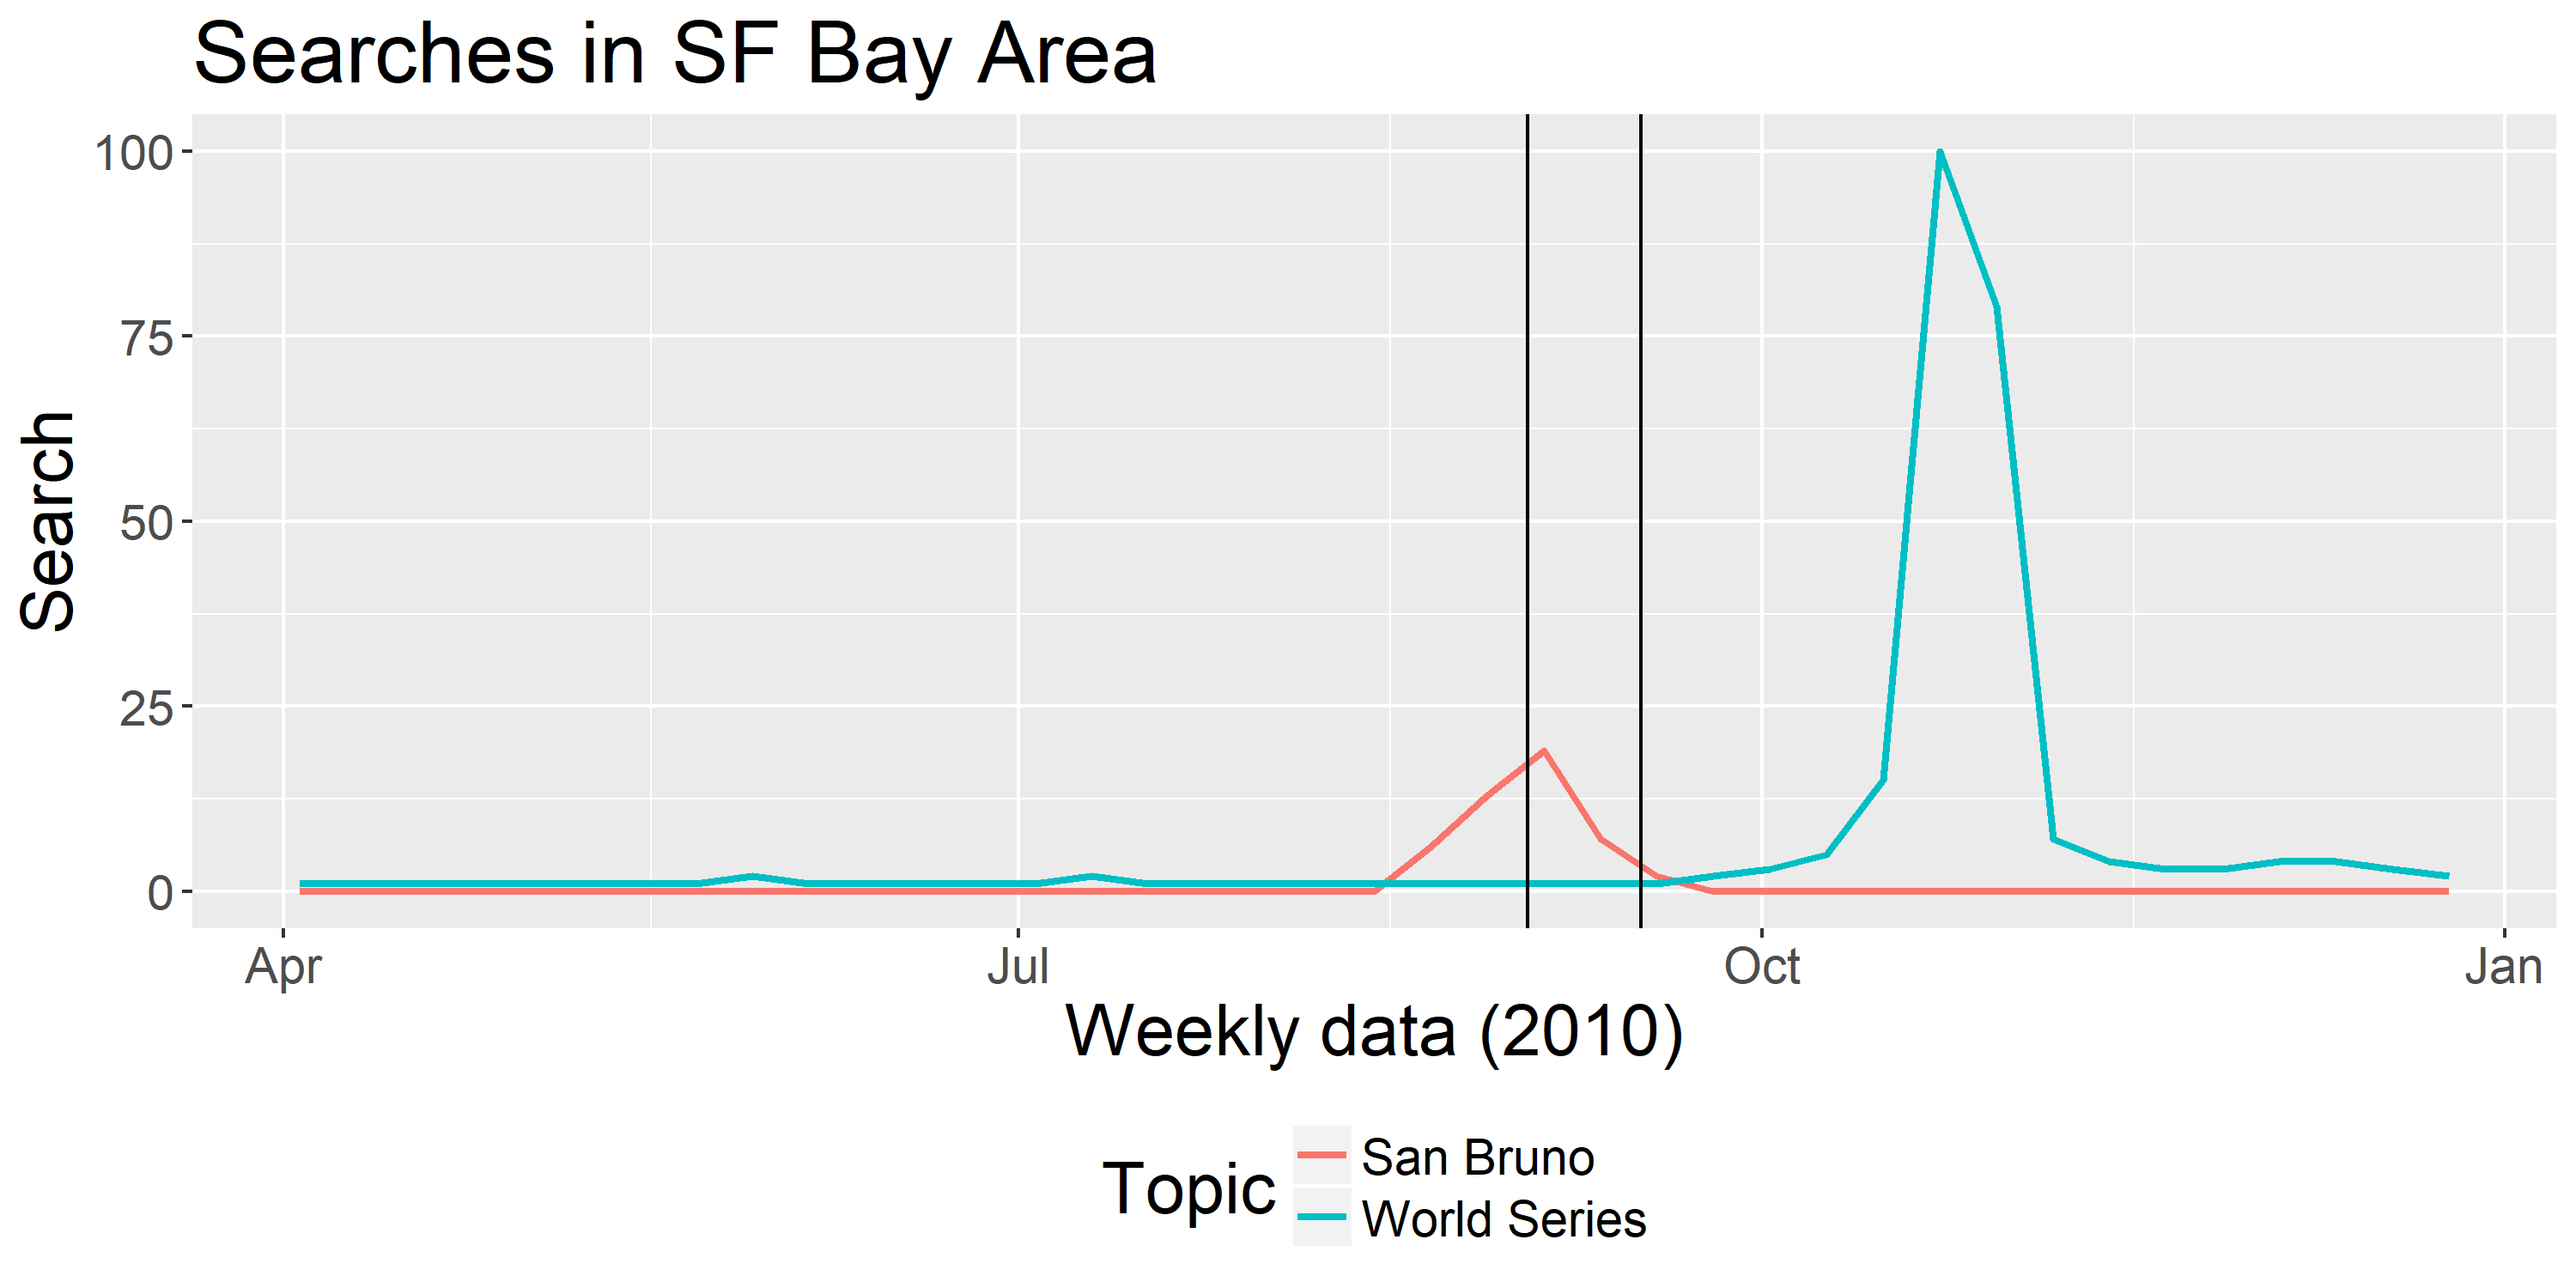
\includegraphics[width=0.75\textwidth]{../output/google_worldseries_web.png}
\par\end{centering}
\footnotesize Figures show weekly relative search rates related to
the ``San Bruno Pipeline Explosion'' event and the ``World Series''
as determined by Google algorithm.
\end{figure}

We cannot observe absolute search activity, but we can compare the
San Bruno event to another group of stories thought to be important
to Bay Area residents. In the second graph, we compare the San Bruno
explosion search rate to that for stories related to the Major League
Baseball World Series, which was won by the San Francisco Giants in
October 2010. Searches related to San Bruno were roughly 20\% of the
peak search activity related to the Giants' Series win, suggesting
that pipeline-related coverage and information acquisition were substantial.

By Spring 2011, regulatory pressure led PG\&E to send letters to customers
living within 2000 feet of a natural gas transmission pipeline. These
letters (presented in Appendix Figure \ref{fig:letter}) noted the
tragic nature of the San Bruno explosion, informed the resident that
they lived within 2000 feet of a pipeline, provided a link to their
online pipeline location map and the National Pipeline Mapping System
(NPMS), and outlined some of the new safety measures that PG\&E was
implementing. The letter did not give residents any detailed information
about their specific distance to the pipeline, or the location of
that nearest pipeline. According to the local real estate community,
this letter could be considered ``knowledge of material fact'',
which technically requires the homeowner to disclose this information
to any potential buyer.\footnote{This issue was raised in a press release by a real estate disclosure
firm (http://www.firstamsms.com/content/natural-gas-pipelines-now-disclosed-1),
and confirmed by Kate Konschnik of the Harvard Environmental Law Clinic
\citep{kate_konschnik_personal_2016}.} An important detail is that if a transmission pipeline is near \textendash{}
but not actually encroaching \textendash{} the property, there is
otherwise no requirement to disclose this information to a potential
buyer.\footnote{As of July 1, 2013, all contracts for the sale of residential real
property in California must contain a specified notice pertaining
to gas and hazardous liquid transmission pipelines (California AB
1511, year 2012). However, this notice simply informs the buyer that
pipelines exist (not necessarily near the property), and that they
should go to the NPMS to find out if there is one nearby. It does
not discriminate on the basis of actual pipeline proximity in any
way. Unfortunately, our housing data ends prior to this law going
into effect.} We discuss the implications of this disclosure ambiguity in Section
\ref{sec:Discussion}.

\section{Data\label{sec:Data}}

To study the impact of the San Bruno events, we combine data on housing
transactions with a map of pipeline locations. We purchased detailed
GIS shapefiles of pipeline infrastructure from S\&P Global Platts,
a private firm that specializes in data related to energy and other
heavy industry. These maps provide us with a snapshot of all natural
gas pipelines in the state of California, as of October 2015. We observe
the owner of the pipeline segment, and (in some cases) the parent
pipeline's name and the segment's diameter. As our policy questions
and treatments relate to transmission pipelines, we take measures
to pare the pipeline map down to segments that are most likely used
for transmission purposes.\footnote{Specifically, we drop any pipe from a system with a name that indicates
distribution activity or if the diameter is known to be less than
6 inches. We also drop a pipe if the diameter is missing, unless it
has information about the system it belongs to or is an interstate
pipeline. Our results are very similar using the full network of pipelines.
} Although we cannot independently verify this, Platts claims that
these maps are highly accurate, coding all but two segments in the
shapefile as being within 40 feet (78\% of all pipeline segments in
the sample) or within 165 feet.

We combine this pipeline map with information on all housing transactions
in the state of California from January 1996 - June 2012. The data
come from DataQuick (now a part of CoreLogic), a firm that aggregates
and produces housing data from markets across the United States. In
addition to information on the parties and transaction price, the
data contain information on the the exact street address and accompanying
geolocation, and housing characteristics such as year built, square
footage, number of rooms, number of bathrooms, the presence of a pool,
and the presence of a garage. The housing characteristics are observed
once \textendash{} they are the most recent assessment at the time
the data were collected for our purposes. Similar data have been used
in many hedonic applications in the last several years \citep[e.g.,][]{muehlenbachs_housing_2015}.

\subsection{Sample construction \label{subsec:Sample-construction}}

Like the rest of the United States, California's housing market experienced
a sharp correction in late 2008. Figure \ref{fig:price_trends} plots
the average log housing price by month for houses near and far away
from pipelines. Our identifying events occur in the immediate aftermath
of that crash. Thus, although we obtained house price data going back
to 1996, in our empirical analysis we restrict our sample to begin
on June 16, 2009, after the housing market began to recover and 450
days prior to the San Bruno explosion. In Section \ref{sec:Empirical-strategy},
we discuss strategies to address related potential threats to identification.

\begin{figure}[H]
\caption{California house price trends \label{fig:price_trends}}
\centering{}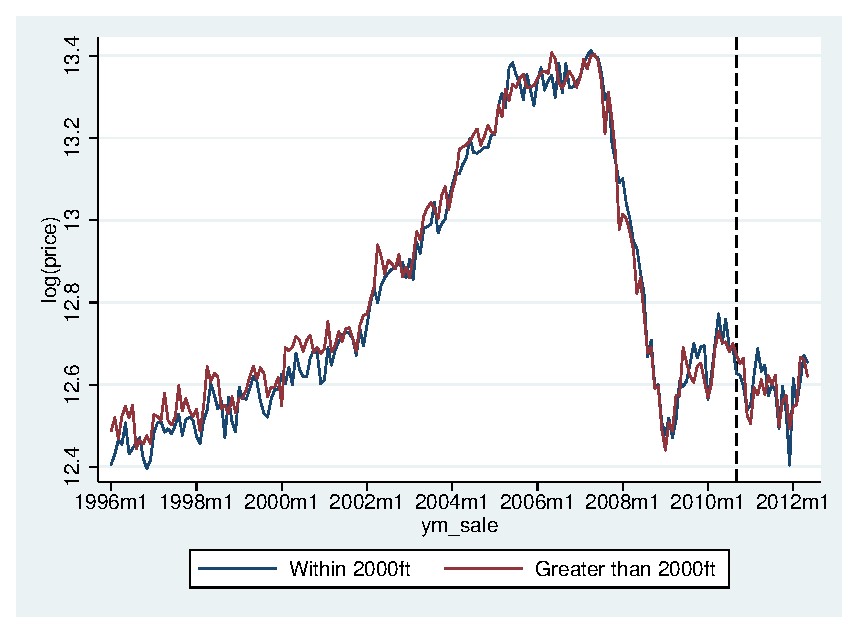
\includegraphics[width=0.6\textwidth]{../output/price_trend_full_sample.eps}
\end{figure}

We then take a number of steps to ensure that our dataset contains
only valid, arms-length transactions that reflect the valuation of
potential homeowners. We drop any transactions that are flagged as
non-arms length transfers, are non-residential properties, mobile
homes, and those whose addresses could not be mapped to a valid latitude
and longitude. In each year, we drop transactions with prices in the
top and bottom one percent. Finally, we drop properties that sell
more than five times in our 16-year dataset, properties with more than
five bedrooms or bathrooms, transactions in which the buyer appeared
to be a corporate entity, and transactions that took place less than
one year since the previous sale. Our main DD specification restricts
the sample to counties that are unambiguously serviced by PG\&E, excluding
any homes within 1 kilometer of the site of the San Bruno explosion.\footnote{These counties are Alameda, Amador, Butte, Calaveras, Colusa, Contra
Costa, Glenn, Humboldt, Lake, Marin, Mariposa, Mendocino, Merced,
Monterey, Napa, Sacramento, San Benito, San Francisco, San Joaquin,
San Mateo, Santa Clara (excluding Palo Alto, which is serviced by
a municipal utility), Santa Cruz, Solano, Sonoma, Stanislaus, Sutter,
Tehama, Tuolumne, Yolo, and Yuba.} Table \ref{tab:sample_obs} reports the number of transactions by
time period and distance group after making these sample restrictions. 

\begin{table}[H]
\caption{Sample observations by time-period and distance to nearest pipeline
\label{tab:sample_obs}}

\centering

\begin{center}
\begin{tabular}{lccc}
\hline \noalign{\smallskip} & 0-1000 & 1000-2000 & 2000-4000\\
\noalign{\smallskip}\hline Pre & 19,467 & 17,871 & 26,784\\
Post-Exp. & 8,817 & 7,940 & 12,043\\
\noalign{\smallskip}Post-Letter & 16,302 & 14,419 & 21,483\\
\noalign{\smallskip}\hline\end{tabular}\\
\end{center}


\scriptsize

The ``Pre'' period includes sales from June 16, 2009 up until the
day before San Bruno. The explosion period (``Post-Exp'') runs from
September 9, 2010 to April 20, 2011 when the PG\&E letters were sent.
The ``Post-Letter'' period runs from that date until the end of
the sample, June 30, 2012. 
\end{table}

\subsection{Descriptive statistics}

A fundamental concern with using house price differentials to infer
latent preferences for avoiding pipelines is that pipelines are not
located randomly. Figure \ref{fig:overlap} plots histograms of covariates
for houses 0-2000 and 2000-4000 feet from the nearest pipeline. The
overall distribution of these variables is generally quite similar
across the two bins, with substantial overlap. Table \ref{tab:summhouses}
formalizes this by regressing each covariate on distance bin dummies
and census tract fixed effects. Houses within 1000-2000 feet of a
pipeline are generally more similar than houses within 1000 ft to
the 2000-4000 ft. control bin. Relative to the sample means, these
differences are modest, but they should be pointed out. Houses near
pipelines tend to be slightly smaller, less likely to have a pool
or garage, and were more likely to be sold under some measure of foreclosure
distress. Although our difference-in-difference approach should alleviate
most concerns, we also allow for rich local trends as well as recent
local foreclosure activity. 

\begin{figure}[H]
\caption{Housing characteristic support by distance from pipeline\label{fig:overlap}}
\centering{}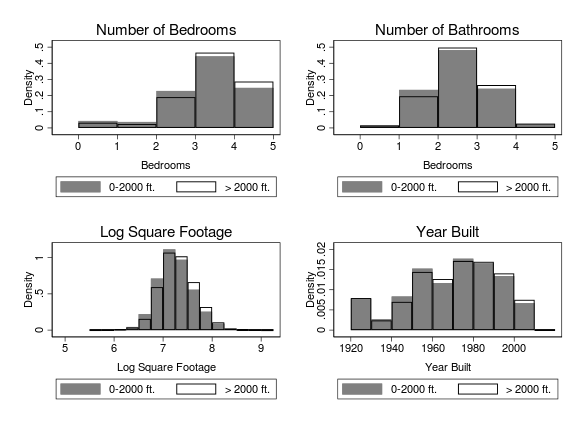
\includegraphics[width=0.8\textwidth]{../output/overlap_bw}
\end{figure}
\begin{table}[H]
\caption{Housing transaction summary statistics\label{tab:summhouses}}

\centering \footnotesize

{
\def\sym#1{\ifmmode^{#1}\else\(^{#1}\)\fi}
\begin{tabular}{l*{7}{c}}
\toprule
                    &\multicolumn{1}{c}{(1)}&\multicolumn{1}{c}{(2)}&\multicolumn{1}{c}{(3)}&\multicolumn{1}{c}{(4)}&\multicolumn{1}{c}{(5)}&\multicolumn{1}{c}{(6)}&\multicolumn{1}{c}{(7)}\\
                    &\multicolumn{1}{c}{Price}&\multicolumn{1}{c}{Beds}&\multicolumn{1}{c}{Baths}&\multicolumn{1}{c}{Pool}&\multicolumn{1}{c}{Garage}&\multicolumn{1}{c}{Sq. Ft.}&\multicolumn{1}{c}{Distress}\\
\midrule
1000ft              &    -34549.1***&      -0.091***&      -0.073***&      -0.015***&      -0.025***&       -75.8***&       0.026***\\
                    &    (1267.5)   &    (0.0066)   &    (0.0054)   &    (0.0021)   &    (0.0021)   &      (4.15)   &    (0.0035)   \\
\addlinespace
2000ft              &    -17663.0***&      -0.044***&      -0.041***&     -0.0023   &     -0.0084***&       -38.7***&       0.018***\\
                    &    (1172.6)   &    (0.0061)   &    (0.0050)   &    (0.0019)   &    (0.0019)   &      (3.84)   &    (0.0032)   \\
\midrule
Mean: 2000-4000 ft. &    378874.1   &        3.05   &        2.14   &       0.089   &        0.69   &      1627.8   &        0.59   \\
\bottomrule
\end{tabular}
}


\scriptsize

Coefficients come from a regression of the housing characteristic
on pipeline distance bins and census tract fixed effects.
\end{table}

\section{Empirical strategy \label{sec:Empirical-strategy}}

We begin with a hedonic equation relating house prices to pipeline
proximity, 
\begin{equation}
\ln P_{it}=\alpha_{o}+\gamma_{it}\alpha_{1}Close_{i}+X_{it}\delta+\epsilon_{it}\label{eq:structural}
\end{equation}
where $P_{it}$ is the sale price of house $i$ with characteristics
$X$ at time $t$, and $Close_{i}$ is an indicator for whether the
household is close to a natural gas pipeline. To capture the fact
that home buyers may not be aware of or attentive to pipeline proximity,
we introduce a discount factor $\gamma\in[0,1]$. When people are
imperfectly informed or inattentive ($\gamma<1$), this discounting
attenuates the observed empirical relationship between pipelines and
equilibrium home prices towards zero, limiting our ability to recover
the true, informed, relationship, $\alpha_{1}$, which is the policy
parameter of interest. 

In this paper, we seek to estimate the extent of this attenuation
in California prior to San Bruno. To do this, we employ a difference-in-differences
(DD) approach, comparing properties near a pipeline to those farther
from a pipeline, before and after the explosion and subsequent letter
campaign. 
\begin{equation}
\ln P_{it}=\alpha_{tr}+\mu_{t}+\beta_{Pre}Close_{i}+\beta_{Expl}Close_{i}\times Expl_{t}+\beta_{Letter}Close_{i}\times Letter_{t}+X_{it}\delta+\epsilon_{it}\label{eq:main_DD}
\end{equation}
Where $Expl_{t}$ indicates that the sale happened between 9/9/2010
and 4/20/2011 (the ``post-explosion'' period), $Letter_{t}$ indicates
that the sale happened after 4/20/2011 (the ``post-letter'' period).
30-day time period dummy variables $\mu_{t}$ are constructed such
that they perfectly partition the pre- and post- San Bruno periods.
$\alpha_{tr}$ is a geographic fixed effect for the property's census
tract, which is a relatively homogeneous geographic unit containing
an average of 4000 residents.

An alternative to tract-level fixed effects would be to include property
fixed effects. While this approach would account for any time-invariant house
heterogeneity within census tracts, the downside is that it requires us to restrict the sample to properties that sell
multiple times in the data. As was discussed in Section \ref{subsec:Sample-construction},
the period of interest comes on the heels of a massive housing market
correction, which limits the explanatory power of time invariant unobservables
and hedonic price gradients. The implications of eschewing property
fixed effects are further discussed in Appendix \ref{sec:Property-fixed-effects}. 

It is important to note that this empirical specification does not
allow us to recover the true WTP to avoid living near a pipeline ($\alpha_{1}$)
without additional assumptions.\footnote{As we discuss in Section \ref{subsec:Regression-discontinuity}, we
would require additional assumptions to claim that the capitalization
effect $\alpha_{1}$ equals WTP. } During our sample, the pipeline network is constant, and we are just
looking at changes in price around existing pipelines. To provide
a mapping between Equations \ref{eq:structural} and \ref{eq:main_DD},
let $\gamma_{Pre}$, $\gamma_{Expl}$, and $\gamma_{Letter}$ be the
discount factor households use prior to San Bruno, after the explosion,
and after receiving a letter. Then 
\[
\beta_{Pre}=\gamma_{Pre}\alpha_{1}
\]
\begin{equation}
\beta_{Explosion}=(\gamma_{Expl}-\gamma_{Pre})\alpha_{1}\label{eq:betaExpl}
\end{equation}
\begin{equation}
\beta_{Letter}=(\gamma_{Letter}-\gamma_{Pre})\alpha_{1}\label{eq:betaLetter}
\end{equation}
This means that even if we assume $\gamma_{Letter}=1$, we cannot
recover the full effect, $\alpha_{1}=\beta_{pre}+\beta_{Letter}$
, without assuming away any time invariant unobservables that are
correlated with pipeline proximity and house prices. As we showed
in Section \ref{sec:Data}, this is unlikely to be the case. Thus,
instead of recovering $\alpha_{1}$, our goal is to consistently estimate
the change in pipeline aversion following the explosion and letter
campaign. We further discuss the interpretation of $\beta_{Explosion}$
and $\beta_{Letter}$ in Section \ref{sec:Discussion}. 

Consistent estimation of $\beta_{Explosion}$ and $\beta_{Letter}$
requires the assumption of parallel trends: absent the San Bruno events,
the difference in unobserved price drivers between properties near
and far from pipelines would have remained constant. To lend credibility
to this assumption we restrict the sample to properties within 4000
feet of a natural gas pipeline. We define $Close_{i}$ to be indicators
if the property is within 1000 feet of the nearest pipeline or between
1000 and 2000 feet from the nearest pipeline. The control group is
houses between 2000 and 4000 feet from the nearest pipeline. 

We also take several steps to account for the fact that these identifying
events occur in the aftermath of an unprecedented housing crash. It
is known that there were systematic local trends in the housing market
during this time driven by factors like foreclosure activity \citep{campbell_forced_2011}.
First, we include very fine space-time fixed effects: tract-specific
period dummies and tract-specific quarter dummies, where periods line
up with our DD periods. This approach allows census tracts to flexibly
differ in their recoveries from the crash. Second, we flexibly control
for foreclosure activity. If there is any indication that a sale involved
a property in distress, we control for the nature of this distress.
In another robustness check, we control for the number of foreclosure
sales that occurred within one-quarter mile of the sale in the previous
six months. This operates as a highly localized measure of the severity
of the housing crisis and recovery, while also accounting for the
potential spillover effects of neighboring foreclosures \citep{campbell_forced_2011,anenberg_estimates_2014}.

\subsection{Regression discontinuity\label{subsec:Regression-discontinuity}}

Recent work has raised concerns about using difference-in-difference strategies to identify hedonic models \citep{banzhaf_panel_2015,kuminoff_capitalization_2014}. In particular, \citet{banzhaf_panel_2015} shows that the DD estimator is a lower bound on the true equivalent surplus associated with an amenity change. We cannot directly address this concern for our entire analysis. However, the letter sent by PG\&E lends itself to a regression discontinuity design (RDD), which exploits only cross-sectional variation rather than relying on parallel trends and a time-invariant hedonic equilibrium. Specifically, we are able to compare houses on either side of the 2000 foot mailing cutoff and test whether housing prices change at that threshold. We follow the suggestion of \citet{imbens_regression_2008} and take a local linear approach within a relatively narrow bandwidth. The sample is further restricted to only house sales after the letters were distributed and only properties between 1000 and 3000 feet from a pipeline. We then control for separate linear functions on either side of the cutoff, and estimate whether there is a jump at 2000 feet. 

Formally, we estimate:
\begin{align}
\ln P_{it}= & \alpha_{0}+\beta_{0}(d_{i}-2000)+\beta_{Letter}^{RD}*(-1)(d_{i}>2000)+\beta_{1}(d_{i}-2000)*(d_{i}>2000)\label{eq:rdd}
\end{align}
where $d_{i}$ is the distance from the property to the nearest natural gas transmission pipeline. Assuming that no other unobservables change discontinuously at this cutoff, the estimate $\beta_{Letter}^{RD}$ reflects the causal effect of letter receipt. We multiply the discontinuity at 2000 feet by (-1) so that the sign on this coefficient matches that of our DD estimator. The main weakness is that the estimated effect is a local average treatment effect at 2000 feet, which is outside the blast zone of any existing pipeline. Still, this provides a test of whether information conveyed by the letter, along with follow-up information acquisition, affected housing prices. 

\section{Results \label{sec:Results}}

\subsection{Difference-in-differences}

We begin by presenting the estimates from Equation \ref{eq:main_DD} in Table \ref{tab:pgeddbase}. The sample is restricted to households living within 4,000 feet of a natural gas pipeline and living in a county served by PG\&E. All specifications include month of sample dummies and controls for housing and transaction characteristics.\footnote{These characteristics are the number of bedrooms and bathrooms, log of square footage, presence of a pool, presence of a garage, type of property (e.g., single-family vs. condo), 10-year bins of property age at time of sale, and dummies for categories of distress.} Moving from left to right in Table \ref{tab:pgeddbase}, the specifications in Columns 1 through 4 include increasingly fine controls for spatial and temporal unobservables. Column 1 contains time-invariant tract fixed effects. In Column 2, tracts are partitioned into properties 0-1000, 1000-2000, and 2000-4000 feet from the nearest pipeline, and a time-invariant control is included for each tract-distance group. In Column 3, the tract fixed effects are interacted with DD time period indicators. Column 4 interacts the tract fixed effects with quarter-of-sample dummies, where quarters are defined as three consecutive 30-day sample windows.

\begin{table}[tbh]
\caption{Difference-in-difference estimates: housing prices\label{tab:pgeddbase}}

%\centering
\footnotesize
\begin{centering}
{
\def\sym#1{\ifmmode^{#1}\else\(^{#1}\)\fi}
\begin{tabular}{l*{7}{c}}
\toprule
                    &\multicolumn{1}{c}{(1)}   &\multicolumn{1}{c}{(2)}   &\multicolumn{1}{c}{(3)}   &\multicolumn{1}{c}{(4)}   &\multicolumn{1}{c}{(5)}   &\multicolumn{1}{c}{(6)}   &\multicolumn{1}{c}{(7)}   \\
\midrule
1000ft              &     -0.0384***&               &     -0.0380***&     -0.0377***&     -0.0335***&     -0.0354***&     -0.0330***\\
                    &   (0.00523)   &               &   (0.00521)   &   (0.00542)   &   (0.00784)   &   (0.00823)   &   (0.00493)   \\
\addlinespace
2000ft              &     -0.0152***&               &     -0.0156***&     -0.0159***&    -0.00725   &    -0.00922   &     -0.0138***\\
                    &   (0.00383)   &               &   (0.00385)   &   (0.00397)   &   (0.00567)   &   (0.00595)   &   (0.00376)   \\
\addlinespace
PostExp-1000ft      &    -0.00202   &    -0.00150   &   -0.000766   &    -0.00173   &    -0.00886   &    -0.00746   &   -0.000954   \\
                    &   (0.00441)   &   (0.00430)   &   (0.00517)   &   (0.00532)   &   (0.00673)   &   (0.00682)   &   (0.00521)   \\
\addlinespace
PostExp-2000ft      &    0.000804   &     0.00177   &     0.00134   &     0.00137   &    -0.00858   &    -0.00644   &     0.00108   \\
                    &   (0.00390)   &   (0.00386)   &   (0.00436)   &   (0.00458)   &   (0.00608)   &   (0.00637)   &   (0.00442)   \\
\addlinespace
PostLetter-1000ft   &     0.00467   &     0.00473   &     0.00166   &     0.00405   &    -0.00328   &    0.000704   &     0.00238   \\
                    &   (0.00450)   &   (0.00441)   &   (0.00467)   &   (0.00495)   &   (0.00608)   &   (0.00642)   &   (0.00468)   \\
\addlinespace
PostLetter-2000ft   &    0.000267   &    0.000532   &   -0.000897   &    0.000983   &     -0.0101*  &    -0.00674   &   -0.000904   \\
                    &   (0.00380)   &   (0.00377)   &   (0.00394)   &   (0.00415)   &   (0.00557)   &   (0.00581)   &   (0.00395)   \\
\midrule
Tract FEs           &          Tr   &     Tr-Dist   &      Tr-Per   &        Tr-Q   &      Tr-Per   &        Tr-Q   &      Tr-Per   \\
Bay Area            &               &               &               &               &           X   &           X   &               \\
Add'l. Covars.      &               &               &               &               &               &               &           X   \\
Observations        &      145091   &      144948   &      144929   &      143212   &       81549   &       80599   &      144929   \\
R-Squared           &       0.922   &       0.927   &       0.926   &       0.934   &       0.906   &       0.916   &       0.926   \\
\bottomrule
\end{tabular}
}

\par\end{centering}
\scriptsize

The dependent variable in each regression is log house price. All models contain month of sample dummies and housing characteristic controls. Standard errors clustered by census tract are reported in parentheses. 
\end{table}

The results are quite stable across specifications. The main effect on the distance bins reveal that properties within 1000 and 2000 feet of a pipeline are worth about 3\% and 1.5\% less, respectively, than properties within the same tract 2000 to 4000 feet away. However, as discussed above, these estimates are also picking up any unobserved neighborhood and housing characteristics correlated with pipeline presence.\footnote{It is interesting to note that these result differ from other cross-sectional studies referenced by FERC (INGAA,2016\nocite{interstate_natural_gas_association_of_america_pipeline_2016};\citealp{fruits_impact_2008}). Those studies typically find no correlation between house prices an pipelines either in in cross-sectional regression or in a ``comparables'' study carried out by appraisers. } Turning to the coefficients of interest ($\beta_{Expl}$ and \textbf{$\beta_{Letter}$}), there is no evidence across any of the models that this difference in home value changed after either the explosion or the subsequent informational letter. Taking Column 3 as an example, the average price effect of the explosion on houses within 1000 feet of a pipeline is -0.07\%, with a 95\% confidence interval of {[}-1.05\%, 0.91\%{]}. 

The remaining three columns in the table present robustness results. Columns 5 and 6 are analogous to Columns 3 and 4, except that we restrict the sample to the ``core Bay Area'' counties of Alameda, Contra Costa, Marin, San Francisco, San Mateo, and Santa Clara. In Column 7, we turn back to the full PG\&E sample with tract-period fixed effects, but also control for the number of foreclosures within one-quarter mile in the six months preceding the sale and the distance to nearest highway interacted with our DD periods. The results for the Bay Area only sample are small and not statistically different from zero as well. However, the point estimates are slightly larger than our estimates for the full PG\&E territory, although they are not statistically distinguishable from one another. This difference may represent statistical noise, or some hint of a response in the area closest to the explosion. In Column 7, the additional covariates meant to capture highly localized market trends do not have an appreciable effect on our estimates.

\subsection{Triple difference}

One possible concern with the difference-in-differences strategy is
divergent trends. There could be price trends in other neighborhood
characteristics that are correlated with pipeline locations, perhaps
due to the housing crisis, that would confound our estimates. While
we cannot directly test for this, we run a triple-difference estimator
where we use Southern California as a control group. Equation \ref{eq:main_DD}
becomes: 
\begin{eqnarray}
\ln P_{it} & = & \alpha_{tr}+\mu_{t}+X_{it}\delta+\beta_{Pre}Close_{i}+\beta_{Expl}Close_{i}\times Expl_{t}+\beta_{Letter}Close_{i}\times Letter_{it}\nonumber \\
 &  & +PGE_{i}\times[\beta_{Pre}^{PGE}Close_{i}+\beta_{Expl}^{PGE}Close_{i}\times Expl_{t}+\beta_{Letter}^{PGE}Close_{i}\times Letter_{it}]+\epsilon_{it}\label{eq:ddd}
\end{eqnarray}
where $PGE_{i}$ denotes that the property is in PG\&E's service territory.
Now $\beta_{Expl}^{PGE}$ and $\beta_{Letter}^{PGE}$ are the coefficients
of interest. In this specification, $\beta_{Expl}^{PGE}$ and can
be interpreted in one of two ways. First, if we assume there is no
San Bruno explosion effect outside of PG\&E territory, then this can
be interpreted as the full effect. Otherwise, we can interpret it
as the differential impact of the media coverage in Northern California
and see if there is a raw difference-in-difference effect in Southern
California. As there was no letter sent in the spring/summer of 2011
in Southern California, $\beta_{Letter}^{PGE}$ should represent the
causal price effect under the normal triple-difference identification
assumptions.

The results from the triple-difference specification are given in
Table \ref{tab:triple_diff}. Columns 1 and 2 present the triple-difference
results using PG\&E territory as the area of interest, with Southern
California Gas and San Diego Gas and Electric service territories
as a control group. Again, we find no impact on prices, and can rule
out even modest price decreases. Columns 3 and 4 restrict the Northern
California sample to the Bay Area, and use only Los Angeles and Orange
Counties as the control group. We find that the treatment effect in
the Bay Area is very close to zero when measured relative to trends
in the Los Angeles area.

\begin{table}[H]
\caption{Triple difference estimates: housing prices\label{tab:triple_diff}}

%\centering
\footnotesize
\begin{centering}
{
\def\sym#1{\ifmmode^{#1}\else\(^{#1}\)\fi}
\begin{tabular}{l*{4}{c}}
\toprule
                    &\multicolumn{1}{c}{(1)}   &\multicolumn{1}{c}{(2)}   &\multicolumn{1}{c}{(3)}   &\multicolumn{1}{c}{(4)}   \\
\midrule
PostExp-1000ft      &    -0.00707   &    -0.00578   &    -0.00883*  &    -0.00832   \\
                    &   (0.00438)   &   (0.00450)   &   (0.00532)   &   (0.00548)   \\
\addlinespace
PostExp-2000ft      &    -0.00402   &    -0.00414   &    -0.00468   &    -0.00640   \\
                    &   (0.00415)   &   (0.00428)   &   (0.00506)   &   (0.00529)   \\
\addlinespace
PostExp-1000ft-PGE  &     0.00599   &     0.00387   &    0.000387   &     0.00139   \\
                    &   (0.00682)   &   (0.00701)   &   (0.00866)   &   (0.00884)   \\
\addlinespace
PostExp-2000ft-PGE  &     0.00490   &     0.00502   &    -0.00453   &   -0.000686   \\
                    &   (0.00603)   &   (0.00628)   &   (0.00796)   &   (0.00833)   \\
\addlinespace
PostLetter-1000ft   &    -0.00431   &    -0.00283   &    -0.00824*  &    -0.00747   \\
                    &   (0.00374)   &   (0.00397)   &   (0.00465)   &   (0.00499)   \\
\addlinespace
PostLetter-2000ft   &     0.00307   &     0.00347   &   -0.000814   &    -0.00161   \\
                    &   (0.00342)   &   (0.00360)   &   (0.00429)   &   (0.00453)   \\
\addlinespace
PostLetter-1000ft-PGE&     0.00602   &     0.00724   &     0.00528   &     0.00873   \\
                    &   (0.00604)   &   (0.00640)   &   (0.00772)   &   (0.00821)   \\
\addlinespace
PostLetter-2000ft-PGE&    -0.00402   &    -0.00252   &    -0.00942   &    -0.00525   \\
                    &   (0.00525)   &   (0.00552)   &   (0.00705)   &   (0.00739)   \\
\midrule
Tract FEs           &      Tr-Per   &        Tr-Q   &      Tr-Per   &        Tr-Q   \\
Bay Area            &               &               &           X   &           X   \\
Observations        &      320028   &      313995   &      206604   &      202215   \\
R-Squared           &       0.918   &       0.928   &       0.900   &       0.913   \\
\bottomrule
\end{tabular}
}

\par\end{centering}
\scriptsize

The dependent variable in each regression is log house price. All
models contain month of sample dummies and housing characteristic
controls. Standard errors clustered by census tract are reported in
parentheses. 
\end{table}

\subsection{Quarterly treatment effects}

The previous regressions failed to find any evidence of a permanent shift in the hedonic price gradient after the explosion or the letter. However, it is possible that these shocks to awareness were more fleeting. In order to test for shorter impacts, we also perform an event study-style regression. That is, we allow the difference-in-difference treatment effects to vary by quarter.\footnote{The results are similar if we estimate monthly treatment effects rather than quarterly effects.} \emph{A priori}, we do not know how long it should take for the effects of the explosion or letter to arise in equilibrium prices.\emph{ }For example, the letter campaign was announced in a press release and subsequent news coverage on April 20, 2011. However, we do not know the exact rollout dates of these letters, and attempts to obtain them from PG\&E or the California Public Utilities Commission have been unsuccessful.\footnote{The limited news coverage we found indicates that Berkeley residents received letters during the last week of June 2011, while Napa residents received them in mid-July. } This specification can be written as:

\begin{equation}
\ln P_{it}=\alpha_{tr}^{q}+\mu_{t}+\sum_{q}\beta_{Qtr}^{q}Close_{i}\times Qtr_{t}^{q}+X_{it}\delta+\epsilon_{it}\label{eq:qtr_DD}
\end{equation}
where $\alpha_{tr}^{q}$ is census tract-quarter fixed effect and
$Qtr_{t}^{q}$ is a indicator for whether $t$ in the 90 day sample
period $q$. $\beta_{Qtr}^{q}$ is therefore the quarterly average
difference between properties near and far from pipelines within the
same census tract. 

The results are presented in Figure \ref{fig:Quarterly-treatment-effects}.
The solid black line denotes the date of the San Bruno explosion.
The dashed black vertical lines represent the announcement of the
PG\&E letter campaign (4/20/2011, which defines the beginning of the
``Letter'' period in the DD specification) and the latest date of
letter receipt we could find in the media (7/21/2011 in Napa, CA).
The dotted lines are 95\% confidence intervals. There is no discernable
pattern in the quarterly estimates for either bin over time.
\begin{center}
\begin{figure}[H]
\begin{centering}
\caption{Quarterly treatment effects \label{fig:Quarterly-treatment-effects}}
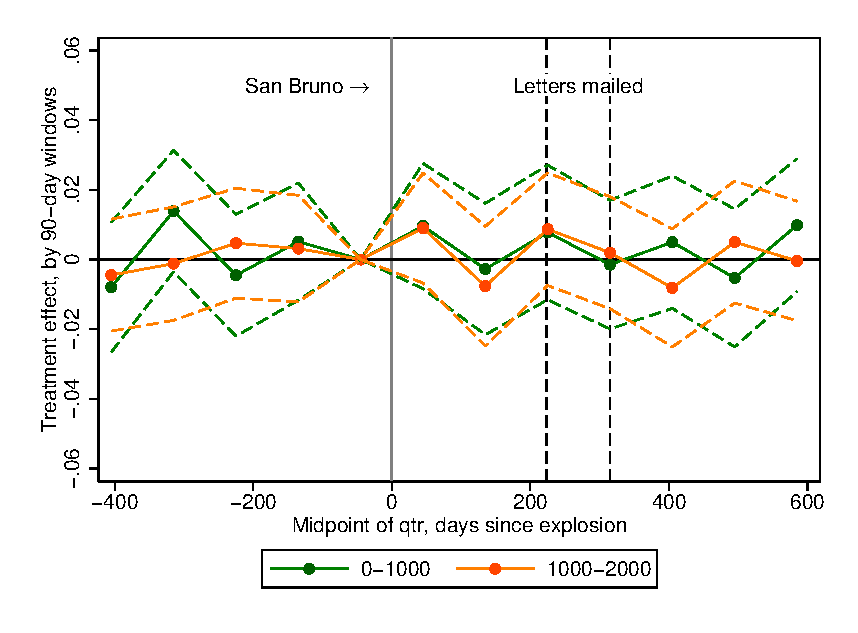
\includegraphics[width=0.7\textwidth]{../output/PGE_xs_qtr_TrQtr}
\par\end{centering}
\centering \scriptsize Dotted lines are 95\% confidence intervals
derived from standard errors clustered by census tract.
\end{figure}
\par\end{center}

\subsection{Regression discontinuity}

Before turning to the regression discontinuity estimates, it is useful
to examine the the price data around the discontinuity visually. Figure
\ref{fig:Graphical-RD-results} presents the binned mean log(price)
values along with 95 percent confidence intervals within 1000 feet
of the letter cutoff.\footnote{This plot was created with the rdrobust package from Calonico et.
al., available at \href{https://sites.google.com/site/rdpackages/}{https://sites.google.com/site/rdpackages/}.} Visually, there is no clear evidence of a discontinuity. 

\begin{figure}[H]
\caption{Graphical RD results\label{fig:Graphical-RD-results}}
\centering{}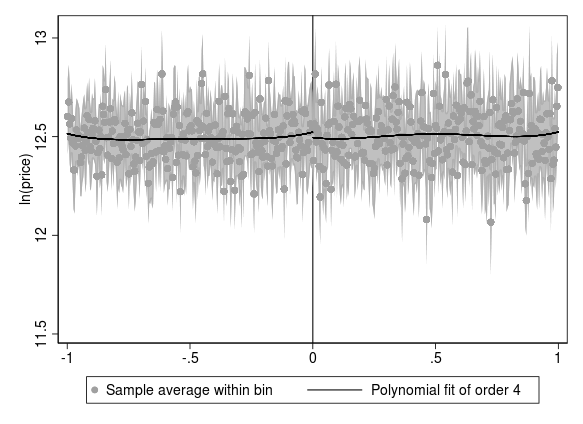
\includegraphics[width=0.75\textwidth]{../output/rdplot_pge_lnprice}
\end{figure}

Table \ref{tab:rd-results} confirms this visual interpretation using
the linear regression from Equation \ref{eq:rdd}. Column 1 presents
the results where the only controls included are month dummies. The
point estimate implies that houses just within the letter radius are
0.2\% \emph{more }valuable than houses just outside the radius that
were not sent a letter. Column 2 and 3 add in tract dummies and housing
characteristic controls. Column 4 narrows the bandwidth further to
include just households within 1,500 and 2,500 of a PG\&E pipeline.
In all four models, $\beta_{Letter}^{RD}$ is statistically indistinguishable
from zero. 

\begin{table}[H]
\caption{Regression discontinuity results \label{tab:rd-results}}

%\centering
\footnotesize
\begin{centering}
{
\def\sym#1{\ifmmode^{#1}\else\(^{#1}\)\fi}
\begin{tabular}{l*{4}{c}}
\toprule
                    &\multicolumn{1}{c}{(1)}   &\multicolumn{1}{c}{(2)}   &\multicolumn{1}{c}{(3)}   &\multicolumn{1}{c}{(4)}   \\
\midrule
RD\_Estimate         &     0.00206   &     0.00902   &    -0.00851   &      0.0146   \\
                    &    (0.0195)   &   (0.00869)   &   (0.00586)   &    (0.0119)   \\
\midrule
Bandwidth           &     1000 ft   &     1000 ft   &     1000 ft   &      500 ft   \\
Hedonics            &               &               &           X   &               \\
TractFEs            &               &           X   &           X   &           X   \\
Observations        &       26309   &       26309   &       26309   &       13069   \\
\bottomrule
\end{tabular}
}

\par\end{centering}
The dependent variable in each model is log(price), and all models
include month of sale dummies. Robust standard errors presented in
parentheses. 
\end{table}

\section{Discussion\label{sec:Discussion}}

What do these results tell us about willingness to pay to avoid natural gas pipeline risk? As was discussed in Section \ref{sec:Empirical-strategy}, the answer depends on the magnitude of $(\gamma_{Expl}-\gamma_{Pre})$ and $(\gamma_{Letter}-\gamma_{Pre})$. The background evidence presented above suggests $\gamma_{Pre}$ was well below one prior to the explosion. Coverage lamenting lack of information was ubiquitous, and even first responders were uninformed about pipeline locations. Moreover, the PG\&E letter mailing was prompted precisely because awareness was so low. 

While it seems safe to assume $\gamma_{Pre}$ was close to zero, taking a stand on the change in $\gamma$ after the explosion and letter is more difficult. This was a major national news story, garnering days of coverage on nightly news programs, and coverage persisted much longer in California. As the Google search data shows, many of those living Northern California also turned to the internet for information on pipelines at a rate never seen before. While we cannot relate this directly to the number of homebuyers affected, let alone their priors, it seems reasonable to assume that this bump in attention was considerable. 

Turning to the change in $\gamma$ from the letter, this is also tough to gauge. On the one hand, this is about as powerful an information treatment as we could imagine implementing at scale. PG\&E compiled a list of all residents living within a relatively large area around each of its pipelines. It then sent millions of residents a concise letter invoking the still salient tragedy of San Bruno, alerting them of their situation, and directing them to a website for more information. Like all mailers, we have no way of knowing how many of these letters were opened and internalized. 

A potentially larger limitation of the letter treatment is that the information was only given to homeowners, not buyers. As was discussed above, there is conflicting information over whether this was a legally material fact that should be disclosed when closing. Regardless of the literal letter of the law, we doubt that this disclosure often happened in practice. Instead, we interpret any change in $\gamma$ as coming from coverage of the letters and word of mouth, rather than from a formal disclosure process. Given this, it is important to note the distinction between this paper and earlier disclosure work by \citet{pope_buyer_2008}, which focused on disclosure laws explicitly mandating disclosure to potential buyers.

If we assume that the shock to $\gamma$ from either the explosion or the letter was significant, then our results suggest even a fully informed housing market would reveal little willingness to pay to avoid pipeline safety risk. This is consistent with fully informed households having rational expectations about this small risk. We can invert the standard VSL formula to back out an implied willingness to pay to avoid this risk. 
\[
MWTP=VSL\times PiplineRisk
\]
Between 1996 and 2015, there were 12 fatalities from natural gas transmission pipeline incidents in California (including San Bruno). In the CoreLogic data, 28\% of CA households are within 2000 feet of a transmission
pipeline, which implies an annual pipeline risk of 0.053 deaths per million people. Using the current EPA VSL figure of \$8.5M, this implies an annual willingness to pay of just \$1.32 per household.

How can we relate this revealed rational apathy to the safety-based arguments made in opposition to new pipelines? One possible reconciliation is preference heterogeneity. If the most concerned households have already sorted, then the loss in utility from pipelines that encroach into new areas may be steep, even if the gradient near old pipelines appears flat. An alternative explanation for this apparent disconnect between stated and revealed concern is NIMBYism. New pipelines do impose some distinct disamenities on local communities, particularly during construction or when eminent domain is invoked to create a new right-of-way. These affected parties may realize that messages related to pipeline safety are particularly effective at drumming up community and political support.\footnote{For example, a 2018 editorial in the Boston Globe decried, ``Pipelines have been embraced as a convenient environmental bogeyman, blamed for everything from inviting enemy attack to the imminent incineration of West Roxbury, and politicians have been unable to see past the hyperbole.'', \textit{The Boston Globe}, 7/14/2018.}

In some cases it is clear that pipeline protests ostensibly focused on concerns tied to a specific location are primarily fueled by more global concerns about hydraulic fracturing or climate change.\footnote{Most notably, opposition to the Keystone and Dakota Access Pipelines} While all global externalities associated with hydrocarbon extraction and consumption should be considered by policymakers, masking these concerns under the guise of local causes can inflate infrastructure costs at little social value.\footnote{As one example, the 2017 state budget adopted in densely-populated Massachusetts included a provision prohibits all new fossil fuel transmission pipelines "located in an area which is less than 1 mile in linear distance from a playground, licensed day-care center, school, church, area of critical environmental concern, ..., or an area occupied by residential housing prohibits any pipelines near schools or senior centers" (Massachusetts Budget Amendment ID: FY2017-S4-931).} 

Finally, it should be noted that efforts to increase pipeline awareness and information availability may still be valuable, even if they do not have a large effect on housing choices on the margin. Accurate information allows those living near pipelines to make safety plans and respond accordingly should another disaster like San Bruno occur. In the event that our estimates obscure a small share of the population with very high willingness to pay to avoid pipelines, information provision should also aid efficient sorting.  Thus, pipeline information campaigns may be valuable for these reasons, even if they are unlikely to alter housing market equilibrium. 

\section{Conclusion \label{sec:Conclusion}}

Safety concerns are a major impediment to making necessary expansions to the natural gas pipeline network. While there appears to be very little revealed willingness to pay to avoid existing natural gas pipelines, it is difficult to know if this reflects true ambivalence or simply a lack of salience and awareness. In this paper, we attempt to resolve this ambiguity by studying the fallout from the San Bruno disaster, which shocked both salience and information. Using multiple identification strategies, we fail to to find any evidence of a meaningful shift in the hedonic price gradient following these events. While efforts to raise information and salience may still be valuable, these results suggest their absence are not obscuring some large latent aversion to pipelines.

\section*{\protect\pagebreak{}}

%\bibliographystyle{plainnat}
%\bibliography{HS_pipelines}

\printbibliography

\section*{\protect\pagebreak{}}


\appendix
\pdfbookmark{Appendix A - Data Appendix}{Anchor A}

\setcounter{figure}{0}  \renewcommand{\thefigure}{A.\arabic{figure}} 
\setcounter{table}{0}  \renewcommand{\thetable}{A.\arabic{table}} 

\section{Additional figures}

\begin{figure}[H]
\caption{Map of San Bruno Damage\label{fig:sanbruno}}
\begin{centering}

\includegraphics[width=1\textwidth]{../images/SanBrunoFireMap.pdf}
\par\end{centering}
\centering{}\footnotesize Source: City of San Bruno (https://sanbruno.ca.gov/civicax/filebank/blobdload.aspx?blobid=22862)
\end{figure}

\begin{figure}[H]
\caption{PG\&E Sample Letter\label{fig:letter}}
\begin{centering}
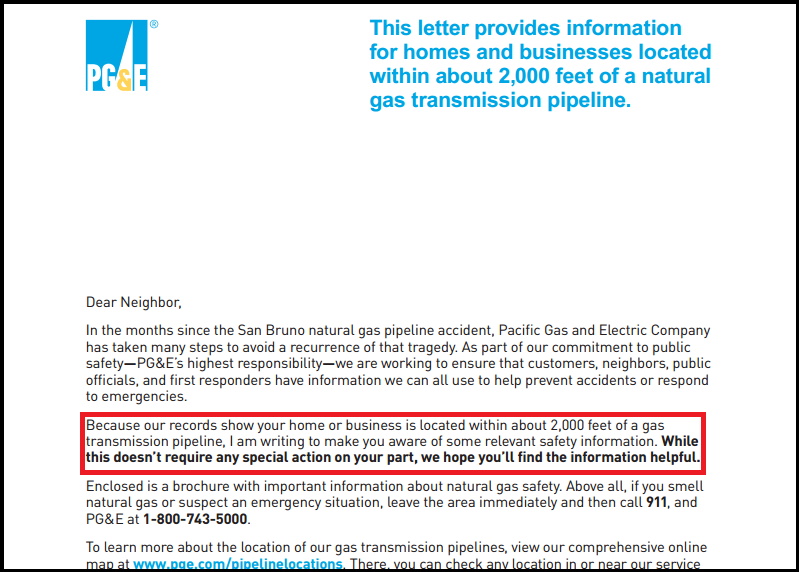
\includegraphics[width=1\textwidth]{../images/PGE_letter.png}
\par\end{centering}
\centering{}\footnotesize Source: City of San Bruno (https://sanbruno.ca.gov/civicax/filebank/blobdload.aspx?blobid=22862)
\end{figure}

\section{Property fixed effects \label{sec:Property-fixed-effects} }

\setcounter{figure}{0}  \renewcommand{\thefigure}{B.\arabic{figure}} 
\setcounter{table}{0}  \renewcommand{\thetable}{B.\arabic{table}} 

One potential concern with our approach is that we are not sufficiently controlling for unobservable housing characteristics that are correlated with pipeline proximity. Given that our housing data stretches back to 1996, property fixed effects allow us to examine this concern. The housing market equilibrium has clearly changed substantially during and after the housing crisis. Thus, we do not want to use data stretching back that far as our ``pre'' period. Unfortunately, restricting ourselves to four years of repeat sales data both reduces our sample considerably, and also introduces severe sample selection problems.

Instead, we use the full sample, but include a ``double-difference'' term for the period before 6/16/2009. We want to compare the post-explosion period to a reference period that is relatively stable. This approach ``removes'' the data generated in the pre-crash market equilibrium from directly ``helping'' to estimate the treatment effect. We still leave this data in because it allows us to use property fixed effects in some specifications without losing all of our data (or selecting on properties that sell twice during 2009-2012). We estimate the following specification:

\begin{align}
\ln P_{it}= & \alpha_{i}+\mu_{t}+\beta_{Pre}Close_{i}+\beta_{PC}Close_{i}\times PreCrash_{t}+\beta_{Expl}Close_{i}\times Expl_{t}+\label{eq:pfe}\\
 & \beta_{Letter}Close_{i}\times Letter_{it}+X_{it}\delta+\epsilon_{it}\nonumber 
\end{align}
which is identical to Equation \ref{eq:main_DD}, except that we now include property fixed effects $\alpha_{i}$ and the extra ``Pre-crash'' DD term. We present the results of Equation \ref{eq:pfe} in Table \ref{tab:pfe}. Comparing Column 1 to Column 2 and Column 3 to Column 4, it is clear that accounting for unobservable time-invariant housing characteristics has very little effect on the difference-in-difference estimates.

\begin{table}[H]
\caption{Difference-in-difference estimates with property fixed effects: housing
prices\label{tab:pfe}}

%\centering
\footnotesize
\begin{centering}
{
\def\sym#1{\ifmmode^{#1}\else\(^{#1}\)\fi}
\begin{tabular}{l*{4}{c}}
\toprule
                    &\multicolumn{1}{c}{(1)}   &\multicolumn{1}{c}{(2)}   &\multicolumn{1}{c}{(3)}   &\multicolumn{1}{c}{(4)}   \\
\midrule
PostExp-1000ft      &    -0.00138   &     0.00403   &    -0.00916   &    -0.00279   \\
                    &   (0.00723)   &   (0.00891)   &   (0.00757)   &   (0.00889)   \\
\addlinespace
PostExp-2000ft      &     0.00270   &     0.00295   &     0.00173   &     0.00718   \\
                    &   (0.00675)   &   (0.00839)   &   (0.00666)   &   (0.00799)   \\
\addlinespace
PostLetter-1000ft   &      0.0104   &     0.00743   &    -0.00684   &    -0.00740   \\
                    &   (0.00690)   &   (0.00829)   &   (0.00628)   &   (0.00677)   \\
\addlinespace
PostLetter-2000ft   &     0.00139   &     0.00366   &    -0.00508   &    0.000230   \\
                    &   (0.00631)   &   (0.00755)   &   (0.00572)   &   (0.00645)   \\
\midrule
Property FE         &           N   &           Y   &           N   &           Y   \\
Other FE            &          Tr   &               &      Tr-Per   &      Tr-Per   \\
Observations        &      509859   &      509859   &      509487   &      509243   \\
R-Squared           &       0.863   &       0.934   &       0.882   &       0.948   \\
\bottomrule
\end{tabular}
}

\par\end{centering}
\scriptsize

The dependent variable in each regression is log house price. All models contain month of sample dummies and housing characteristic controls. Standard errors clustered by census tract are reported in parentheses. 
\end{table}

\end{document}